\documentclass{article}
\usepackage{tikz}
\usepackage{float}
\usepackage{amsmath}
\usepackage{bm}
\usepackage[utf8]{inputenc}

\title{8.01 V-Groove Problem}
\author{Robert Durfee}
\date{November 3, 2017}

\begin{document}

\maketitle

A cylinder of mass $m$ and radius $R$ is rotated in a V-groove with constant angular velocity $\omega$. The coefficient of friction between the cylinder and the surface is $\mu$. What external torque must be applied to the cylinder to keep it rolling at a constant angular speed?
\begin{figure}[H]
    \centering
    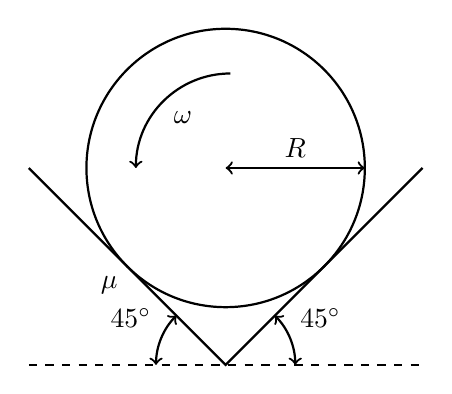
\begin{tikzpicture}
        \draw [thick] (-2.5,2.5) -- (0,0) -- (2.5,2.5);
        \draw [thick] (0,2.5) circle (1.76777);
        \draw [thick, ->] (0.06,3.7) arc (90:180:1.2) node[pos=0.5, anchor=north west]{$\omega$};
        \draw [thick, dashed] (-2.5,0) -- (2.5,0);
        \draw [thick, <->] (-0.625,0.625) arc (135:180:0.88388) node[pos=0.5, anchor=south east]{$45^{\circ}$};
        \draw [thick, <->] (0.625,0.625) arc (45:0:0.88388) node[pos=0.5, anchor=south west]{$45^{\circ}$};
        \draw [thick, <->] (0.0,2.5) -- (1.76777,2.5) node[pos=0.5, anchor=south]{$R$};
        \fill [] (-1.25,1.25) circle (0pt) node[anchor=north east]{$\mu$};
    \end{tikzpicture}
\end{figure}

Identify all forces acting on the cylinder.
\begin{figure}[H]
    \centering
    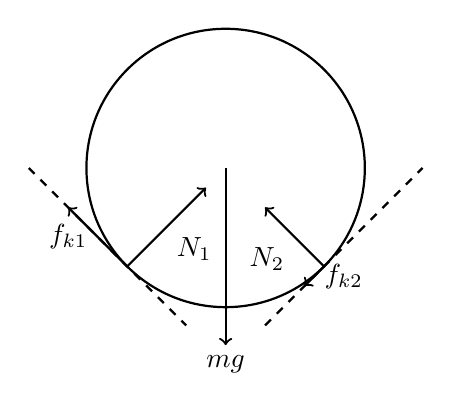
\begin{tikzpicture}
        \draw [thick, dashed] (-2.5,2.5) -- (-0.5,0.5);
        \draw [thick, dashed] (0.5,0.5) -- (2.5,2.5);
        %\fill [] (0,2.5) circle (1.5pt);
        \draw [thick] (0,2.5) circle (1.76777);
        \draw [thick, ->] (-1.25,1.25) -- (-2,2) node[pos=0.5, anchor=east]{$f_{k1}$};
        \draw [thick, ->] (1.25,1.25) -- (1.00,1.00) node[pos=0.5, anchor=west]{$f_{k2}$};
        \draw [thick, ->] (0,2.5) -- (0, 0.25) node[pos=1, anchor=north]{$mg$};
        \draw [thick, ->] (-1.25,1.25) -- (-0.25,2.25) node[pos=0.5, anchor=north west]{$N_{1}$};
        \draw [thick, ->] (1.25,1.25) -- (0.50,2.00) node[pos=0.5, anchor=north east]{$N_{2}$};
    \end{tikzpicture}
\end{figure}

Draw a free-body diagram for the cylinder.
\begin{figure}[H]
    \centering
    \begin{tikzpicture}
        \fill [] (0,0) circle (2pt);
        \draw [thick, ->] (0,0) -- (0,-2) node[pos=1, anchor=north east]{$mg$};
        \draw [thick, ->] (0,0) -- (1.41421,1.41421) node[pos=1, anchor=north west]{$N_{1}$};
        \draw [thick, ->] (0,0) -- (-1.2,1.2) node[pos=1, anchor=north east]{$N_{2}$};
        \draw [thick, ->] (0,0) -- (-0.5,-0.5) node[pos=1, anchor=north east]{$f_{k2}$};
        \draw [thick, ->] (0,0) -- (-0.707107,0.707107) node[pos=1, anchor=south west]{$f_{k1}$};
        \draw [thick, ->] (4,0) -- (3.5,0.5) node[pos=1, anchor=south east]{$+\hat{j}$};
        \draw [thick, ->] (4,0) -- (4.5,0.5) node[pos=1, anchor=south west]{$+\hat{i}$};
    \end{tikzpicture}
\end{figure}

Then resolve the free-body diagram within the coordinate system.
\begin{figure}[H]
    \centering
    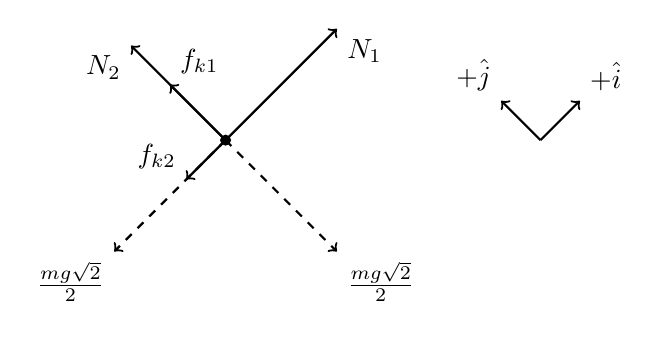
\begin{tikzpicture}
        \fill [] (0,0) circle (2pt);
        \draw [thick, ->] (0,0) -- (1.41421,1.41421) node[pos=1, anchor=north west]{$N_{1}$};
        \draw [thick, ->] (0,0) -- (-1.2,1.2) node[pos=1, anchor=north east]{$N_{2}$};
        \draw [thick, ->] (0,0) -- (-0.5,-0.5) node[pos=1, anchor=south east]{$f_{k2}$};
        \draw [thick, ->] (0,0) -- (-0.707107,0.707107) node[pos=1, anchor=south west]{$f_{k1}$};
        \draw [thick, dashed, ->] (0,0) -- (-1.41421,-1.41421) node[pos=1, anchor=north east]{$\frac{mg\sqrt{2}}{2}$};
        \draw [thick, dashed, ->] (0,0) -- (1.41421,-1.41421) node[pos=1, anchor=north west]{$\frac{mg\sqrt{2}}{2}$};
        \draw [thick, ->] (4,0) -- (3.5,0.5) node[pos=1, anchor=south east]{$+\hat{j}$};
        \draw [thick, ->] (4,0) -- (4.5,0.5) node[pos=1, anchor=south west]{$+\hat{i}$};
    \end{tikzpicture}
\end{figure}

Write out Newton's 2nd Law for each direction:
\begin{align*}
    N_{2}+f_{k1}-\frac{mg\sqrt{2}}{2}&=ma_{y}\\
    N_{1}-f_{k2}-\frac{mg\sqrt{2}}{2}&=ma_{x}
\end{align*}

Substitute for the values of kinetic friction:
\begin{align*}
    N_{2}+\mu N_{1}-\frac{mg\sqrt{2}}{2}&=ma_{y}\\
    N_{1}-\mu N_{2}-\frac{mg\sqrt{2}}{2}&=ma_{x}
\end{align*}

Because the cylinder does not accelerate in the $x$ or $y$ direction, $ma=0$:
\begin{align}
    N_{2}+\mu N_{1}-\frac{mg\sqrt{2}}{2}&=0\\
    N_{1}-\mu N_{2}-\frac{mg\sqrt{2}}{2}&=0
\end{align}

Multiply equation 1 by $\mu$ to allow elimination of $N_{2}$:
\begin{align}
    \mu N_{2}+\mu^{2} N_{1}-\frac{\mu mg\sqrt{2}}{2}&=0\\
    N_{1}-\mu N_{2}-\frac{mg\sqrt{2}}{2}&=0
\end{align}

Add equations 3 and 4 together:
\begin{align*}
    \mu N_{2}+\mu^{2} N_{1}-\frac{\mu mg\sqrt{2}}{2}+N_{1}-\mu N_{2}-\frac{mg\sqrt{2}}{2}&=0\\
    \mu^{2} N_{1}-\frac{\mu mg\sqrt{2}}{2}+N_{1}-\frac{mg\sqrt{2}}{2}&=0\\
    \frac{mg\sqrt{2}}{2}+\frac{\mu mg\sqrt{2}}{2}&=\mu^{2} N_{1}+N_{1}\\
    \frac{mg\sqrt{2}}{2}(1+\mu)&=(\mu^{2}+1)N_{1}\\
    \bm{\frac{mg\sqrt{2}}{2}\left(\frac{1+\mu}{\mu^{2}+1}\right)}&\bm{=N_{1}}
\end{align*}

Substitute $N_{1}$ into equation 2:
\begin{align*}
    \left(\frac{mg\sqrt{2}}{2}\frac{(1+\mu)}{(\mu^{2}+1)}\right)-\mu N_{2}-\frac{mg\sqrt{2}}{2}&=0\\
    \left(\frac{mg\sqrt{2}}{2}\frac{(1+\mu)}{(\mu^{2}+1)}\right)-\frac{mg\sqrt{2}}{2}&=\mu N_{2}\\
    \frac{mg\sqrt{2}}{2}\left(\frac{(1+\mu)}{(\mu^{2}+1)}-1\right)&=\mu N_{2}\\
    \frac{mg\sqrt{2}}{2}\left(\frac{(1+\mu)}{\mu(\mu^{2}+1)}-\frac{1}{\mu}\right)&=N_{2}\\
    \bm{\frac{mg\sqrt{2}}{2}\left(\frac{1-\mu}{\mu^{2}+1}\right)}&\bm{=N_{2}}
\end{align*}

Use $N_{1}$ to determine frictional force $f_{k1}$:
\begin{align*}
    f_{k1}&=\mu N_{1}\\
    f_{k1}&=\mu \left(\frac{mg\sqrt{2}}{2}\left(\frac{1+\mu}{\mu^{2}+1}\right)\right)\\
    \bm{f_{k1}}&\bm{=\frac{mg\sqrt{2}}{2}\left(\frac{\mu+\mu^{2}}{\mu^{2}+1}\right)}
\end{align*}

Use $N_{2}$ to determine frictional force $f_{k2}$:
\begin{align*}
    f_{k2}&=\mu N_{2}\\
    f_{k2}&=\mu \left(\frac{mg\sqrt{2}}{2}\left(\frac{1-\mu}{\mu^{2}+1}\right)\right)\\
    \bm{f_{k2}}&\bm{=\frac{mg\sqrt{2}}{2}\left(\frac{\mu-\mu^{2}}{\mu^{2}+1}\right)}
\end{align*}

Write out angular analog for Newton's 2nd Law for the cylinder:
\begin{align*}
    \tau_{ext}-\tau_{fk1}-\tau_{fk2}&=I\alpha\\
    \tau_{ext}-f_{k1}R-f_{k2}R&=I\alpha
\end{align*}

Since we know the cylinder is moving at a constant angular velocity, there is no angular acceleration:
\begin{align*}
    \tau_{ext}-f_{k1}R-f_{k2}R&=0\\
    R\left(f_{k1}+f_{k2}\right)&=\tau_{ext}
\end{align*}

Substitute our values for $f_{k1}$ and $f_{k2}$:
\begin{align*}
    R\left(\frac{mg\sqrt{2}}{2}\left(\frac{\mu+\mu^{2}}{\mu^{2}+1}\right)+\frac{mg\sqrt{2}}{2}\left(\frac{\mu-\mu^{2}}{\mu^{2}+1}\right)\right)&=\tau_{ext}\\
    \frac{Rmg\sqrt{2}}{2}\left(\frac{\mu+\mu^{2}}{\mu^{2}+1}+\frac{\mu-\mu^{2}}{\mu^{2}+1}\right)&=\tau_{ext}\\
    \frac{Rmg\sqrt{2}}{2}\left(\frac{2\mu}{\mu^{2}+1}\right)&=\tau_{ext}\\
    \bm{\frac{Rmg\mu\sqrt{2}}{\mu^{2}+1}}&\bm{=\tau_{ext}}
\end{align*}

\end{document}
